\begin{abcliste}
\abc Auf den Wagenzug wirken die Gewichtskraft $\vec F_\mathrm{G}$ und die Normalkraft $\vec F_\mathrm{N}$ der Schienen (senkrecht zur Bahn, zum Mittelpunkt). Die Zentripetalkraft $F_\mathrm{Z} = \frac{m\,v^2}{r}$ ist die Summe der zum Mittelpunkt zeigenden Komponenten:
\begin{align}
 F_\mathrm{N} - m\,g\cos\alpha &= \frac{m\,v^2}{r}
\end{align}
Für ein massstäbliches Bild braucht man die Geschwindigkeiten. Wir nehmen an, dass der Zug reibungsfrei fährt und oben gerade die Mindestgeschwindigkeit aus (b) hat, $v_\pi^2 = g\,r$. Auf der Höhe $h = r\left(1-\cos\alpha\right)$ über dem tiefsten Punkt gilt dann nach dem Energiesatz
\begin{align}
 v^2 &= v_\pi^2 + 2g\left(2r-h\right) = g\,r\left(3+2\cos\alpha\right)
\end{align}
Damit wird
\begin{align}
 F_\mathrm{Z} &= m\,g\left(3+2\cos\alpha\right), & F_\mathrm{N} &= F_\mathrm{Z} + m\,g\cos\alpha = 3\,m\,g\left(1+\cos\alpha\right)
\end{align}
\begin{center}
\begin{tabular}{c|c|c|c}
 $\alpha$ & Lage & $F_\mathrm{Z}$ & $F_\mathrm{N}$ \\ \hline
 $0$ & unten & $5\,m\,g$ & $6\,m\,g$ \\
 $\pi/2$ & seitlich & $3\,m\,g$ & $3\,m\,g$ \\
 $3\pi/4$ & schräg oben & $\left(\kZcF\right)m\,g \approx \kZcS{2}\,m\,g$ & $\kNcF\,m\,g \approx \kNcS{2}\,m\,g$ \\
 $\pi$ & oben & $m\,g$ & $0$
\end{tabular}
\end{center}
Unten zeigt die Gewichtskraft vom Mittelpunkt weg, die Normalkraft muss sie und zusätzlich die Zentripetalkraft aufbringen. Bei $\alpha = \pi/2$ wirkt die Gewichtskraft tangential (sie bremst nur), die Normalkraft allein ist die Zentripetalkraft. Bei $\alpha = 3\pi/4$ trägt die Komponente $m\,g\cos\left(\pi/4\right)$ der Gewichtskraft zur Zentripetalkraft bei, oben liefert die Gewichtskraft sie allein. In der Skizze (blau: $\vec F_\mathrm{G}$, rot: $\vec F_\mathrm{N}$) ist die Normalkraft unten sechsmal so lang wie die Gewichtskraft:

\begin{center}
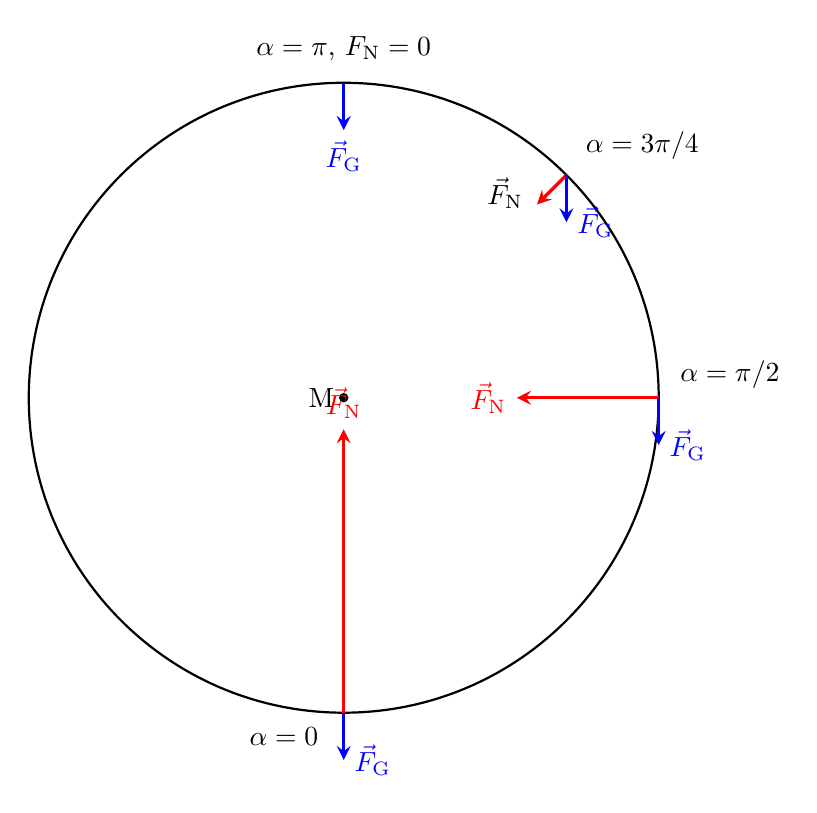
\begin{tikzpicture}[>=stealth]
 \draw[thick] (0,0) circle (4);
 \fill (0,0) circle (0.06) node[left] {M};
 \draw[->, very thick, red] (0,-4) -- (0,-0.4) node[above] {$\vec F_\mathrm{N}$};
 \draw[->, very thick, blue] (0,-4) -- (0,-4.6) node[right] {$\vec F_\mathrm{G}$};
 \node[anchor=east] at (-0.2,-4.3) {$\alpha = 0$};
 \draw[->, very thick, red] (4,0) -- (2.2,0) node[left] {$\vec F_\mathrm{N}$};
 \draw[->, very thick, blue] (4,0) -- (4,-0.6) node[right] {$\vec F_\mathrm{G}$};
 \node[anchor=west] at (4.15,0.3) {$\alpha = \pi/2$};
 \draw[->, very thick, red] (2.828,2.828) -- (2.455,2.455);
 \node[anchor=east] at (2.4,2.6) {$\vec F_\mathrm{N}$};
 \draw[->, very thick, blue] (2.828,2.828) -- (2.828,2.228) node[right] {$\vec F_\mathrm{G}$};
 \node[anchor=south west] at (2.95,2.9) {$\alpha = 3\pi/4$};
 \draw[->, very thick, blue] (0,4) -- (0,3.4) node[below] {$\vec F_\mathrm{G}$};
 \node[anchor=south] at (0,4.15) {$\alpha = \pi$, $F_\mathrm{N} = 0$};
\end{tikzpicture}
\end{center}

\abc Im höchsten Punkt zeigen Gewichtskraft und Normalkraft nach unten. Die kleinste Geschwindigkeit ergibt sich, wenn die Schienen keine Kraft mehr ausüben und die Gewichtskraft allein die Zentripetalkraft liefert: $m\,g = \frac{m\,v^2}{r}$, also
\begin{align}
 v_\mathrm{min} &= \vLpF = \sqrt{\gE\cdot\rLp} = \vLp \approx \result{\vLpP{0}{2}}
\end{align}
\end{abcliste}
